% Milestone 2 report, CSE 216 / COGS 230, Fall 2026. Two pages of text in 11-point Arial; figures after page 2; references on one extra page.
% Build: cd Final_Project/report && tectonic M2_report.tex (needs tectonic; uses ../paper/refs.bib and ../paper/figures).
% Every number here also appears in Final_Project/paper/main.tex or report/M2_draft.md, which name the results file it comes from.
\documentclass[11pt]{article}
\usepackage[margin=1in]{geometry}
\usepackage{fontspec}
\setmainfont{Arial}
\usepackage{graphicx}
\usepackage{float}
\graphicspath{{../paper/figures/}}
\usepackage{enumitem}
\setlist{nosep,leftmargin=1.2em}
\usepackage{titlesec}
\titleformat{\section}{\large\bfseries}{}{0pt}{}
\titlespacing*{\section}{0pt}{8pt}{3pt}
\usepackage[hidelinks]{hyperref}
\setlength{\parindent}{0pt}
\setlength{\parskip}{4pt}
\pagestyle{plain}
\emergencystretch=1.5em

\begin{document}

{\large\bfseries Offloading or Surrendering? Milestone 2 Report}\\
Wayne Wang \textbullet\ CSE 216 / COGS 230, Fall 2026 \textbullet\ solo project

The project asks which patterns of AI use in writing support a writer's thinking (offloading) and which replace it (surrender), and which log signals a tool could act on. Since Milestone 1, AI agents working under my direction have coded and analyzed all 528 request windows and drafted a full paper. Two things did not go as planned: I did not code the data myself, and the scope moved from research writing to formal long-form writing.

\section{1. Current Progress}

\begin{itemize}
  \item \textbf{Data.} An agent's rebuild showed that Milestone 1's 347 NIRVANA windows come from 71 students, not 77 \cite{jelson2026nirvana}. Milestone 1's research-writing sample from WildChat could not be reproduced, so I widened the scope. Under my direction, AI agents screened WildChat \cite{zhao2024} for formal long-form writing and coded 35 conversations (151 windows) from a random seed.
  \item \textbf{Literature.} You asked for a reproducible selection process. Under my direction, AI agents searched OpenAlex and arXiv by script and screened 713 records, with the queries and prompts saved. Google Scholar blocks automated queries, so I still need to run 11 Scholar queries by hand.
  \item \textbf{Framework.} You asked how offloading can be judged in a given scene. Each window is coded on five questions, and a rule table, frozen before new labels were read, maps the codes to one category with a cited source \cite{risko2016,shaw2026}. A category is an inference from behavior, not a measure of thinking.
  \item \textbf{Coding (not as planned).} The proposal said I would be the primary coder. Instead, two AI coders and an AI adjudicator coded every window. Agreement between coders is $\kappa = 0.79$ to 0.94 on the key fields. \textbf{All agreement is AI-to-AI; no human has coded anything.}
  \item \textbf{Success criterion (half met).} The rules assign real windows to categories. But an AI agent's comparison did not show cases that only this framework can separate.
\end{itemize}

\textbf{What the data show so far} (106 sessions; Figures~\ref{fig:concept} and~\ref{fig:signals}). These results rest on AI-coded labels, the timing and paste results come from NIRVANA only, and none is causal.
\begin{itemize}
  \item \textbf{Pasting is not the line.} Writers paste in about 65\% of both support and surrender windows. The difference is what comes after: a median of 6 characters typed after pasting a whole AI answer, against 304.5 after taking part of one. Sessions with more unchecked pasting end with more AI text in the essay ($\rho = 0.60$) and lower felt ownership ($\rho = -0.55$).
  \item \textbf{The writer's own draft is the anchor.} Sessions that start from a visible draft lean to the support side (0.77 support share, against 0.50 with nothing visible).
  \item \textbf{Two log events flag risk without reading the text}: a request on a near-empty page, and a large paste with little typing. Together they catch 63.3\% of surrender-leaning windows.
\end{itemize}


\section{2. Planned Activities (before the final paper, Dec 7)}
\begin{itemize}
  \item \textbf{Add a human check}, because all agreement is AI-to-AI: I will code 20 windows blind and compare with the AI labels.
  \item \textbf{Fix the weakest rule.} Asking for text with no visible use tracks essay outcomes only weakly ($\rho = 0.19$). I will split this rule and rerun.
  \item \textbf{Narrow the contribution claim} to what the data support: telling apart a writer's own claim reworded from an AI claim adopted, on the same act of pasting.
  \item \textbf{Run the 11 Scholar queries}, fold in this meeting's feedback, and submit the revised report by Nov 27.
\end{itemize}

\section{3. Desired Feedback}
\begin{enumerate}
  \item \textbf{How should the paper lead?} Our strongest finding is that pasting is not the line between support and substitution; what the writer does next is. Should the final paper lead with this boundary, or with the two log signals for in-situ feedback?
  \item \textbf{What would make the signals convincing?} Two log-only signals already catch 63.3\% of surrender-leaning windows. Would a held-out test or interface mockups make them more convincing for an HCI audience?
  \item \textbf{Is our human check the right one?} All 528 windows are AI-coded, with AI-to-AI agreement of $\kappa = 0.79$ to 0.94. We plan a blind human check on 20 windows. Is that the right check, or would coding only the disputed cases be stronger?
\end{enumerate}

\begin{figure}[H]
\centering
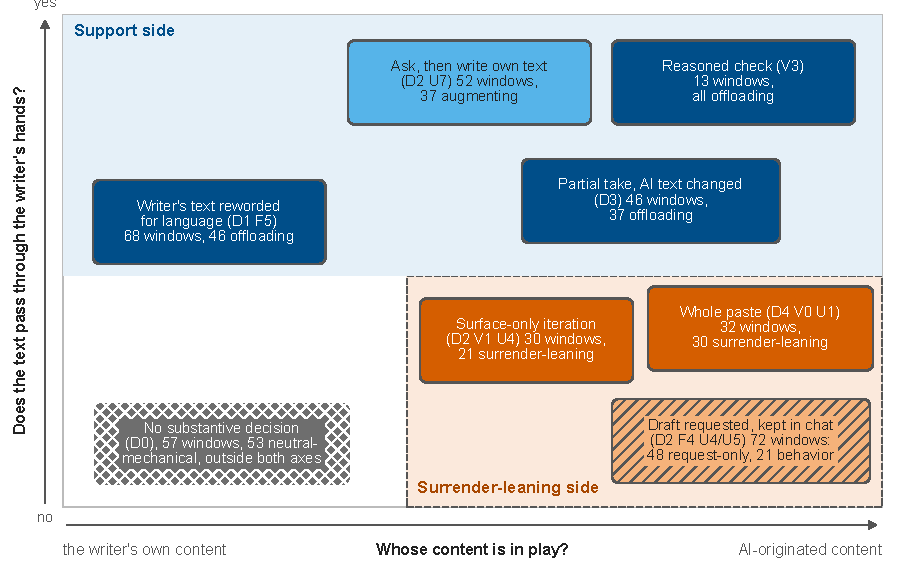
\includegraphics[width=0.6\linewidth]{concept_map.pdf}
\caption{Concept map of the categories. The horizontal axis is whose content it is, and the vertical axis is whether the text passes through the writer's hands. Counts are windows in the 106 whole sessions, coded by AI agents.}
\label{fig:concept}
\end{figure}
\begin{figure}[H]
\centering
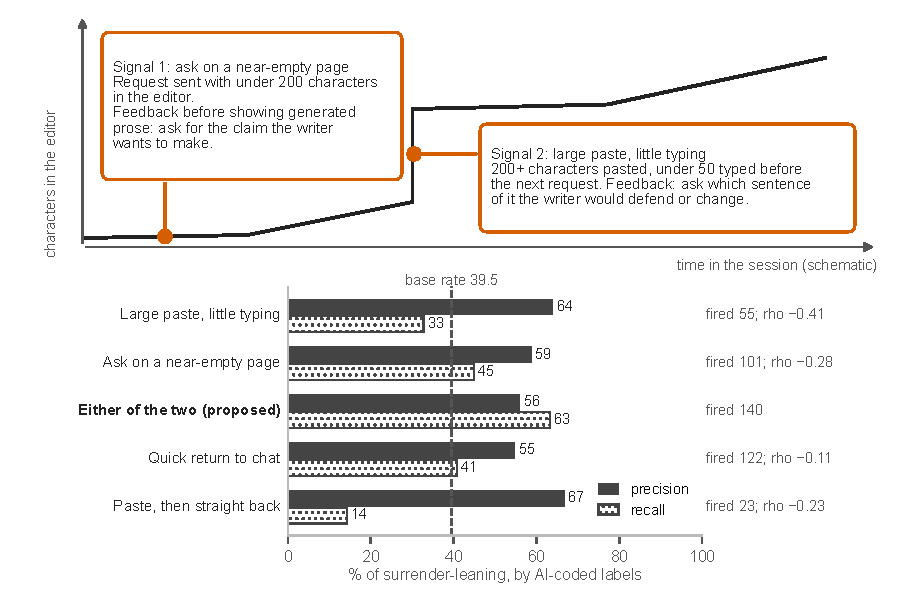
\includegraphics[width=0.6\linewidth]{signals.pdf}
\caption{Top: where the two proposed log signals fire in a session (schematic; nothing was built). Bottom: how often each log-only rule is right (precision) and how many surrender-leaning windows it catches (recall) in NIRVANA's 347 windows, both judged against the AI-coded labels.}
\label{fig:signals}
\end{figure}

\clearpage
\bibliographystyle{plain}
\bibliography{../paper/refs,m2_extra}

\end{document}
